\documentclass{beamer}
\usepackage{tikz}
\usepackage{hyperref}
\usepackage{bm}
\usepackage{booktabs}       % professional-quality tables
\usetheme{metropolis}
\usepackage[utf8]{inputenc}
\usepackage[english]{babel}
\usepackage[T1]{fontenc}
\usepackage{helvet}
\usepackage{amsmath,amsfonts} % Math packages
\usepackage{mathtools}
\usepackage{bbm}
\usepackage{tcolorbox}
\usepackage{standalone}
\usepackage{pgfplots}  % Plots in Latex
%\usepackage{subfig}

\usetikzlibrary{bayesnet}

% Plotting settings for the introduction plots
\pgfplotsset{width=7cm,compat=1.8}
\pgfplotsset{%
  colormap={whitered}{color(0cm)=(white);
  color(1cm)=(orange!75!red)}
}


%-------------------------------------------------------
% DEFFINING AND REDEFINING COMMANDS
%-------------------------------------------------------
\newsavebox{\genericfilt}
\savebox{\genericfilt}{%

\begin{tikzpicture}[font=\small, >=stealth,yscale=0.15,xscale=0.1]
  % define normal distribution function 'normaltwo'
  \def\normaltwo{\x,{exp((-(\x)^2)/0.5)}}
  \draw[line width=0.25mm,domain=-1.7:1.7] plot (\normaltwo);
\end{tikzpicture}%
}

\newsavebox{\genericfiltLarge}
\savebox{\genericfiltLarge}{%
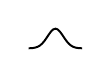
\begin{tikzpicture}[font=\small, >=stealth,yscale=0.25,xscale=0.2]
  % define normal distribution function 'normaltwo'
  \def\normaltwo{\x,{exp((-(\x)^2)/0.5)}}
  \draw[line width=0.25mm,domain=-1.7:1.7] plot (\normaltwo);
\end{tikzpicture}%
}

% colored box for highlighting
\newtcbox{\martinbox}[1][red]{
  on line, 
  %arc=7pt,
  colback=#1!10!white,
  colframe=#1!50!black, 
  before upper={\rule[-3pt]{0pt}{10pt}},
  boxrule=0.5pt, 
  boxsep=0pt,
  left=6pt,
  right=6pt,
  top=2pt,
  bottom=2pt
}

\newtcbox{\martintitlebox}[1][red]{
  %on line, 
  %arc=7pt,
  colback=#1!10!white,
  colframe=#1!50!black, 
  before upper={\rule[-3pt]{0pt}{10pt}},
  boxrule=0pt, 
  boxsep=0pt,
  left=6pt,
  right=6pt,
  top=6pt,
  bottom=6pt
}

% Load definitions
%\newtcolorbox{titlebox}{colback=background,colframe=CBBlue,coltext=gray}
\newtcolorbox{defbox}{colback=white,colframe=gray,coltext=black}

\newcommand{\Categorical}{\ensuremath{\mathcal{C}at}}
\newcommand\Beta{\ensuremath{\mathcal{B}eta}}
\newcommand\Bernoulli{\ensuremath{\mathcal{B}ern}}
\newcommand{\Dirichlet}{\ensuremath{\mathcal{D}ir}}
\newcommand{\Normal}{\ensuremath{\mathcal{N}}}
\newcommand{\Exponential}{\ensuremath{\mathcal{E}xp}}
\newcommand{\Poisson}{\ensuremath{\mathcal{P}oisson}}
\newcommand\DP{\ensuremath{\mathrm{DP}}}
\newcommand\GEM{\ensuremath{\mathrm{GEM}}}
\newcommand{\indpath}[2]{\mathbin{\mathcal{P}{\left(#1,#2\right)}}} % induced path
\newcommand{\indic}{\mathbbm{1}}
\newcommand{\diff}{\mathop{}\!\mathrm{d}}
\newcommand{\SPT}{\mathcal{T}}
\newcommand{\SPG}{\mathcal{C}}
\newcommand{\SPN}{\mathcal{S}}
\newcommand{\graph}{\mathcal{G}}
\newcommand{\ProductNode}{\mathsf{P}}
\newcommand{\ProductNodes}{\bm{\mathsf{P}}}
\newcommand{\SumNode}{\mathsf{S}}
\newcommand{\SumNodes}{\bm{\mathsf{S}}}
\newcommand{\Leaf}{\mathsf{L}}
\newcommand{\Leaves}{\bm{\mathsf{L}}}
\newcommand{\Node}{\mathsf{N}}
\newcommand{\Nodes}{\bm{\mathsf{N}}}
\newcommand{\Child}{\mathsf{C}}
\newcommand{\region}{\ensuremath{R}}
\newcommand{\partition}{\ensuremath{P}}
\newcommand{\regions}{\ensuremath{\mathbf{R}}}
\newcommand{\partitions}{\ensuremath{\mathbf{P}}}
\newcommand{\rg}{\ensuremath{\mathcal{R}}}

\newcommand{\X}{\mathbf{X}}
\newcommand{\data}{\mathcal{X}}
%\newcommand{\x}{\mathbf{x}}
\newcommand{\xn}{\mathbf{x}_{n}}
\newcommand{\xnd}{x_{n,d}}
\newcommand{\xd}{\mathbf{x}_{\cdot,d}}
\newcommand{\Y}{\mathbf{Y}}
\newcommand{\y}{\mathbf{y}}
\newcommand{\yd}{\mathbf{y}}
\newcommand{\ydp}{y_{d,\ProductNode}}
\newcommand{\yndp}{\mathbf{y_{\not{d},\ProductNode}}}
\newcommand{\ydP}{y_{d,\partition}}
\newcommand{\yndP}{\mathbf{y_{\not{d},\partition}}}
\newcommand{\yProduct}{\mathbf{y}_{\cdot,\ProductNode}}
\newcommand{\yPartition}{\mathbf{y}_{\cdot,\partition}}
\newcommand{\Z}{\mathbf{Z}}
\newcommand{\z}{\ensuremath{\mathbf{z}}}
\newcommand{\zn}{\ensuremath{\mathbf{z}_n}}
\newcommand{\zs}{\ensuremath{z_\SumNode}}
\newcommand{\zsn}{\ensuremath{z_{\SumNode,n}}}
\newcommand{\tld}{\ensuremath{\theta_{d,\Leaf}}}


\newcommand{\ks}{\mathbf{k}}
\newcommand{\Root}{\ensuremath{\mathbf{root}}}
\newcommand{\ch}{\ensuremath{\mathbf{ch}}}
\newcommand{\anc}{\ensuremath{\mathbf{anc}}}
\newcommand{\leaf}[1]{\mathbin{\mathbf{leaf}(#1)}} % leaf function
\newcommand{\leafs}[1]{\mathbin{\mathbf{leafs}(#1)}} % leaf function
\newcommand{\w}{w}
\newcommand{\vp}{\mathbf{v}}
\newcommand{\vps}{\mathbf{v}}
%\newcommand{\ws}{\mathbf{w}_{\SumNode}}
\newcommand{\wsc}{w_{\SumNode,\Child}}
\newcommand{\tp}{\mathbf{\theta}}
\newcommand{\val}{\ensuremath{\mathbf{val}}}
\newcommand{\scope}{\psi}
\newcommand{\cond}[2]{\mathbin{\left. #1\nonscript\;\middle|\nonscript\; #2 \right.}}
\newcommand{\cbar}{\,|\,}

\newcommand{\xnew}{\mathbf{x}^{*}}

\newcommand{\argmin}{\arg\!\min} % arg min
\newcommand{\argmax}{\arg\!\max} % arg max

\DeclareMathOperator*{\f}{\SPN(\xn \,|\, \phi)}
\DeclareMathOperator*{\fz}{\SPN(\bm \ast \,|\, \phi)}
\DeclareMathOperator*{\fy}{\SPN(\xn, \lambda_n \,|\, \phi)}
\DeclareMathOperator*{\fzy}{\SPN(\bm \ast, \lambda_n \,|\, \phi)}
\newcommand{\wa}{\w^{[0]}_{\gamma}}
\newcommand{\wb}{\w^{[1]}_{k}}
\newcommand{\wt}{\w^{(t)}_{k}}
\newcommand{\wjt}{\w^{(t)}_{j}}
\newcommand{\wjtt}{\w^{(t+1)}_{j}}
\newcommand{\wtt}{\w^{(t+1)}_{k}}
\newcommand{\wat}{\w^{[0](t)}_{\gamma}}
\newcommand{\wbt}{\w^{[1](t)}_{k}}
\newcommand{\wjbt}{\w^{[1](t)}_{j}}
\newcommand{\watt}{\w^{[0](t+1)}_{\gamma}}
\newcommand{\wbtt}{\w^{[1](t+1)}_{k}}


%-------------------------------------------------------
% INFORMATION IN THE TITLE PAGE
%-------------------------------------------------------

\title[Sum-Product Networks] { Learning Sum-Product~Networks }
\author { Martin Trapp }

\titlegraphic{
  \begin{picture}(0,0)
    \put(350,-200){\makebox(0,0)[rt]{
      
\includegraphics[width=2cm]{TU_Graz} \hspace*{1cm}~
    }}
  \end{picture}
}

\date{}

%-------------------------------------------------------
% THE BODY OF THE PRESENTATION
%-------------------------------------------------------

\begin{document}

%-------------------------------------------------------
% THE TITLEPAGE
%-------------------------------------------------------
\maketitle

%-------------------------------------------------------
% INTRODUCTION
%-------------------------------------------------------

% --
% Introduction on Probabilistic machine learning
% --
\section{Probabilistic Machine Learning}

\frame{
\begin{itemize}
    \item Machine learning: How can we make machines that learn from data?
    \item Probabilistic machine learning: How can we make machines that learn from data using tools from probability theory?
    \item Uncertainty is key to probabilistic machine learning and is expressed in all forms, e.g.~noise in the data, uncertainty over the predictions, uncertainty over the model.
\end{itemize}
}

\frame{
Example: How likely is a traffic jam on highway $X_1$ today?

\begin{itemize}
    \item today = Thursday = $Y = 4$.
    \item Traffic jam model: $\theta$ for all $\{X_i\}_{i=1}^n$ highways in the country.
    \item $p(X_1 = 1, Y = 4 \,|\, \theta) = \int_{X_2} \int_{X_3} \dots \int_{X_n} p(X_1 = 1, Y = 4, X_2 = x_2, X_3 = x_3, \dots, X_n = x_n \, | \, \theta)$
    \item \textbf{We need to be able to marginalise out $X_2, \dots, X_n$ to answer the query.}
\end{itemize}
}

\frame{
    \textbf{Problem:} Probabilistic inference task, such as marginalisation, are often intractable for interesting models.

\begin{table}
\centering
\begin{tabular}{lllll}
             & GANs & VAEs & Flows & SPNs  \\
Sampling     & Y    & Y    & Y     & Y      \\
Density      & N    & N/Y  & Y     & Y      \\
Marginals    & N    & N    & ?     & Y      \\
Conditionals & N    & N    & ?     & Y      \\
Moments      & N    & N    & ?     & Y      \\
MAP          & N    & N    & ?     & N/Y
\end{tabular}
\caption{Robert Peharz, Sum-Product Networks and Deep Learning: A Love Marriage. Talk at ICML, 2019.}
\end{table}
}


% --
% Introduction on Sum-Product Networks
% --
\section{Sum-Product Networks}

\frame{
\begin{itemize}
  \item Sum-product networks (SPNs)\footnote{\scriptsize H. Poon \& P. Domingos: Sum-product networks: A new deep architecture. In UAI, 2011.} is a class of general-purpose probabilistic machine learning models that admit tractable probabilistic inference.
  \item SPNs are a sub-class of so-called tractable probabilistic models or probabilistic circuits.
   \item A class of queries $Q$ on a class of models $M$ is tractable, iff for any query $q \in Q$ and model $m \in M$ the computational complexity is at most polynomial.
  \item SPNs admit many probabilistic inference tasks, such as marginalisation, in linear time in their representation size.
  \end{itemize}
}

\begin{frame}{What is a Sum-Product Network?}
\begin{itemize}
  \item Let $\X = \{X_1, \dots, X_D\}$ be set of $D$ random variables. 
  \item An SPN is a distribution over $\X$ defined as a 4-tuple $\SPN = (\graph, \scope, \w, \tp)$.
  \begin{itemize}
    \item $\graph$ is a computational graph.
    \item $\scope$ is a so-called scope function.
    \item $\w$ denotes the set of sum-weights and $\tp$ the set of leaf node parameters. 
  \end{itemize}
\end{itemize}
 \small This definition\footnote{\scriptsize M. Trapp et al.: Bayesian Learning of Sum-Product Networks. In NeurIPS, 2019.} is conceptually different to the original definitions as it disentangles the computational graph and the scope function.
\end{frame}

\begin{frame}{Computational Graph $\graph$}
 $\graph$ is a rooted connected directed acyclic graph (DAG), containing: sum ($\SumNode$), product ($\ProductNode$) and leaf nodes ($\Leaf$).

\begin{figure}
  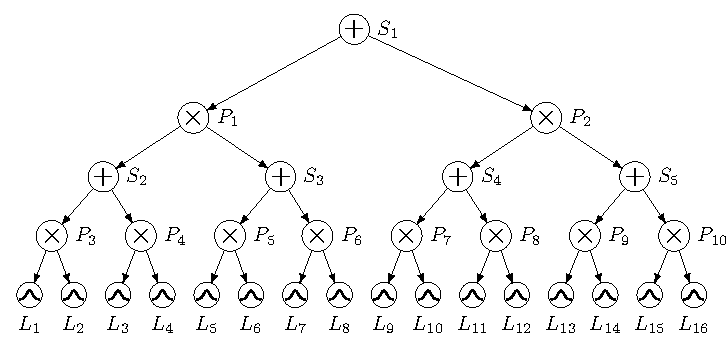
\includegraphics[width=\textwidth]{computation_graph}
  \caption{Example of a tree-shaped computational graph.}
\end{figure}
\end{frame}

\begin{frame}{Leaves $\Leaf$ in $\graph$}
 Leaf nodes are input nodes with arbitrary distribution, e.g.~Gaussian, Multinomial, variational autoencoder.\\[1em]
 
\tikzstyle{vertex}=[inner sep=0.01cm, circle, draw]
\begin{columns}
\begin{column}{.2\linewidth}
\end{column}
\begin{column}{.2\linewidth}
\begin{tikzpicture} [scale=0.5, auto,>=latex,transform shape]
   \node[draw=none](v01) at (1, 1.5) {};
   \node[draw=none](v02) at (-1, 1.5) {};
   \node[vertex](v1) at (0, 0) {\usebox{\genericfiltLarge}};
   \draw [->] (v01) -- (v1);
   \draw [->] (v02) -- (v1);
\end{tikzpicture}
\end{column}
\begin{column}{.4\linewidth}
$\Leaf(x) = p(x \cbar \tp_\Leaf)$
\end{column}
\begin{column}{.2\linewidth}
\end{column}
\end{columns}

\centering
\begin{figure}
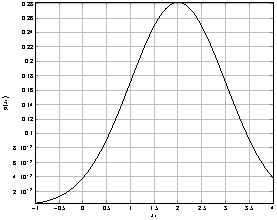
\includegraphics{leaf_distribution}
\end{figure}
\end{frame}

\begin{frame}{Product Nodes $\ProductNode$ in $\graph$}
Product nodes encode independence assumptions between sets of random variables.\\[1em]
 
 \tikzstyle{vertex}=[inner sep=0.01cm, circle, draw]
\begin{columns}
\begin{column}{.2\linewidth}
\end{column}
\begin{column}{.2\linewidth}
\begin{tikzpicture} [scale=0.5, auto,>=latex,transform shape]
   \node[draw=none](v01) at (1, 1.5) {};
   \node[draw=none](v02) at (-1, 1.5) {};
   \node[draw=none](v21) at (1, -1.5) {};
   \node[draw=none](v22) at (-1, -1.5) {};
   \node[vertex](v1) at (0, 0) {\huge$\bm\times$};
   \draw [->] (v01) -- (v1);
   \draw [->] (v02) -- (v1);
   \draw [->] (v1) -- (v21);
   \draw [->] (v1) -- (v22);
\end{tikzpicture}
\end{column}
\begin{column}{.4\linewidth}
$\ProductNode(x)  = \prod\limits_{\Child \in \ch(\ProductNode)} \Child(x)$
\end{column}
\begin{column}{.2\linewidth}
\end{column}
\end{columns}

\centering
\begin{figure}
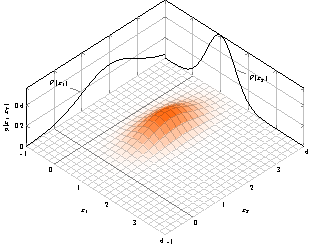
\includegraphics{product_distribution}
\end{figure}
\end{frame}

\begin{frame}{Sum Nodes $\SumNode$ in $\graph$}
Sum nodes\footnote{\scriptsize We assume that $\w_{\SumNode, \Child} \geq 0$ .} replace independence with conditional independence within the network.\\[1em]

\tikzstyle{vertex}=[inner sep=0.01cm, circle, draw]
\begin{columns}
\begin{column}{.2\linewidth}
\end{column}
\begin{column}{.2\linewidth}
\begin{tikzpicture} [scale=0.5, auto,>=latex,transform shape]
   \node[draw=none](v01) at (1, 1.5) {};
   \node[draw=none](v02) at (-1, 1.5) {};
   \node[draw=none](v21) at (1, -1.5) {};
   \node[draw=none](v22) at (-1, -1.5) {};
   \node[vertex](v1) at (0, 0) {\huge$\bm+$};
   \draw [->] (v01) -- (v1);
   \draw [->] (v02) -- (v1);
   \draw [->] (v1) -- (v21);
   \draw [->] (v1) -- (v22);
\end{tikzpicture}
\end{column}
\begin{column}{.4\linewidth}
$\SumNode(x)  = \sum\limits_{\Child \in \ch(\ProductNode)}  \w_{\SumNode, \Child}\Child(x)$
\end{column}
\begin{column}{.2\linewidth}
\end{column}
\end{columns}

\centering
\begin{figure}
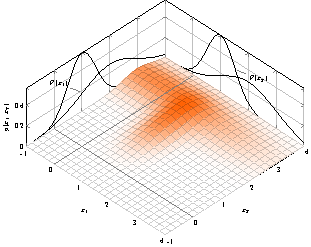
\includegraphics{sum_distribution}
\end{figure}
\end{frame}

\begin{frame}{Scope Function $\scope$}
$\scope$ is a function assigning each node $\Node$ in a sub-set of $\X$,\footnote{\scriptsize This sub-set is often referred to as the scope of a node.} and has to fulfil the following properties: 
\begin{defbox}
\begin{enumerate}
\item If $\Node$ is the root node, then $\scope(\Node) = \X$.
\item If $\Node$ is a sum or product, then $\scope(\Node) = \bigcup_{\Node' \in \ch(\Node)} \scope(\Node')$.
\item For each $\SumNode \in \SumNodes$ we have $\forall \Node, \Node' \in \ch(\SumNode)\colon \scope(\Node) = \scope(\Node')$ (\emph{completeness}) \footnote{\scriptsize Complete and decomposable SPNs are referred to as valid SPNs.}.
\item For each $\ProductNode \in \ProductNodes$ we have $\forall \Node, \Node' \in \ch(\ProductNode)\colon \scope(\Node) \cap \scope(\Node') = \emptyset$ (\emph{decomposability}).
\end{enumerate}
\end{defbox}
\end{frame}

\frame{
\begin{center}Example SPN $\SPN = (\graph, \scope, \w, \tp)$\end{center}
\begin{figure}
  \centering{
    \includestandalone[width=0.9\textwidth]{SPN}
    }
\end{figure}
After applying a scope function $\scope$  on $\graph$ we obtain the SPN. Most structure learners learn both in an entangled way.

\small Note that we define $\Leaf(x):=1$ for every $x$ if and only if $\scope(\Leaf) = \emptyset$.
}


% --
% Parameter learning
% --
\section{Parameter Learning}

\begin{frame}{Parameter Learning in SPNs}{}
\begin{columns}
\begin{column}{\linewidth}
\begin{block}{Generative Learning\footnote{\scriptsize H. Poon \& P. Domingos: Sum-product networks: A new deep architecture. In UAI, 2011.}}
\begin{equation}
  \mathcal{L}(\theta \,| \, \mathcal{X}) = \sum_{n=1}^N \log \f - \log \fz\, , \; \; \xn \in \mathbb{R}^D
\end{equation}
\end{block}
Note that $\fz$ is the partition function which can be evaluated efficiently using a single upward pass.
%\hline
\begin{block}{Discriminative Learning\footnote{\scriptsize R. Gens \& P. Domingos: Discriminative learning of sum-product networks. In NeurIPS, 2012.}}
\begin{equation}
  \begin{aligned}
    \mathcal{L}(\theta, \lambda \,| \, \mathcal{X}) = \sum_{n=1}^N &\log \fy - \log \f\, , \; \; \xn \in \mathbb{R}^D, \, \lambda_n \in \mathbb{R}
\end{aligned}
\end{equation}
\end{block}
\end{column}
\end{columns}
\end{frame}

\begin{frame}{Parameter Learning in SPNs}{}
\begin{block}{Semi-Supervised Learning using Contrastive Pessimistic Likelihood Estimation (CPLE)\footnote{\scriptsize M. Trapp et al.: Safe semi-supervised learning of sum-product networks. In UAI, 2017.}}
\begin{equation}
  \text{CPLE} = \argmax_{\theta \in \Theta} \argmin_{\bm q \in \Delta_{K-1}^M} \mathcal{L}(\theta,  \lambda, \bm{q} \,| \, \mathcal{X}, \mathcal{U}) - \mathcal{L}(\theta^+, \lambda, \bm{q} \,| \, \mathcal{X}, \mathcal{U})
\end{equation}
\end{block}

\begin{figure}
  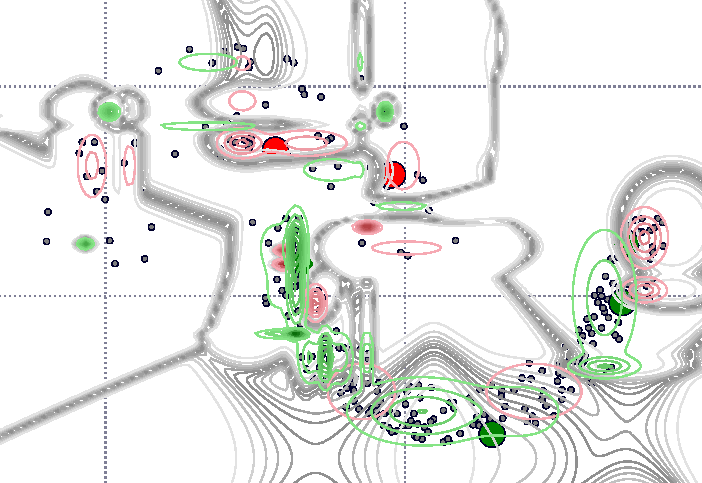
\includegraphics[width=.4\textwidth]{semisupervised_2_2}~
   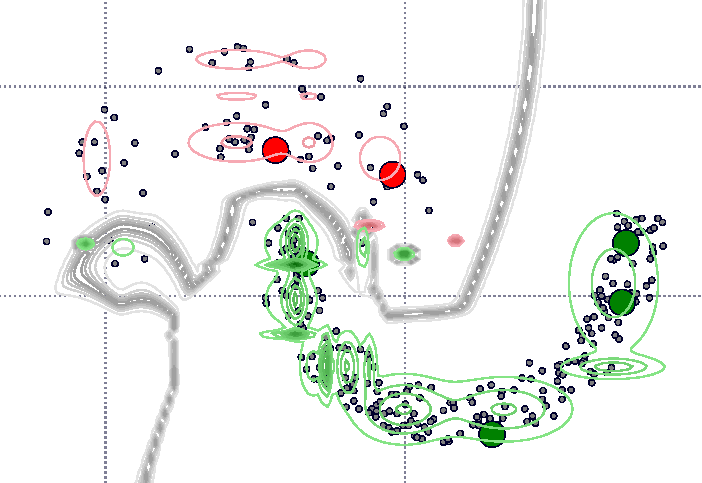
\includegraphics[width=.4\textwidth]{semisupervised_20_2}
\end{figure}

\end{frame}

\begin{frame}{Overparameterization in SPNs\footnote{\scriptsize M. Trapp et al.: Optimisation of Overparametrized Sum-Product Networks. ICML Workshop on Tractable Probabilistic Models, 2019.}}{}
\begin{columns}
\begin{column}{\linewidth}
\begin{align}
    \wt &\approx \wt + \rho^{(t)} \nabla_{\wt} + \left[ \sum_{l=0}^{L-1} \eta \nabla_{w^{[l]}_{\phi(k, l)}} (w^{[l]}_{\phi(k, l)})^{-1} \right] \wt \\
  &= \wt + {\color{cyan} \rho^{(t)}} \nabla_{\wt} + {\color{blue}\sum_{\tau=1}^{t-1} \mu^{(t,\tau)} \nabla_{w^{(\tau)}_k}}
\end{align}\\
  \begin{tcolorbox}[lower separated=false]
  \small{Gradient-based optimisation in deep tree-structured sum-product network with small (fixed) learning rate and near zero initialisation of the weights is equivalent to gradient-based optimisation with adaptive and time-varying {\color{cyan} learning rate} and {\color{blue} momentum term}.}
 \end{tcolorbox}
\end{column}
\end{columns}
\end{frame}

\iffalse
\begin{frame}{Overparameterization in SPNs \small{[Trapp 2019]}}{}
\begin{columns}
\begin{column}{\linewidth}
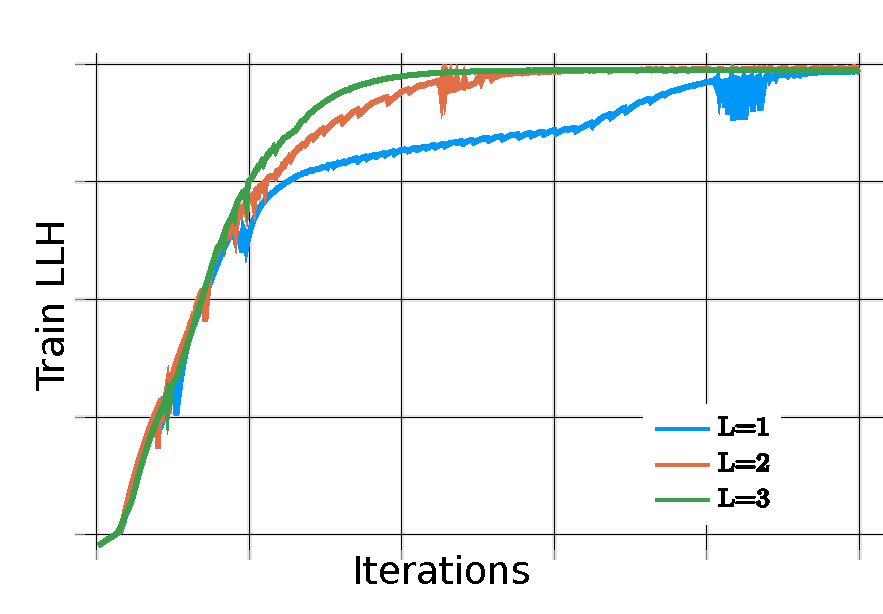
\includegraphics[width=\textwidth]{nltcs_experiment}
\end{column}
\end{columns}
\end{frame}
\fi

\begin{frame}{Bayesian Parameter Learning}
  \begin{itemize}
    \item The key insight for Bayesian parameter learning\footnote{\scriptsize Zhao et al.: Collapsed variational inference for sum-product networks. In ICML, 2016.}
        is that \emph{sum nodes} can be interpreted as \emph{latent variables} $Z_\SumNode$, clustering data instances.
    \item Given a vector of states for each sum, $\z$ induces a so-called induced tree ($\SPT$) on $\SPN$.
  \end{itemize}
  \begin{figure}
  \centering{
    \includestandalone[width=0.7\textwidth]{InducedTree}
    }
\end{figure}
\end{frame}

%\begin{frame}{Bayesian Parameter Learning}
%  \begin{itemize}
%    \item It is now conceptually straightforward to extend an SPN to a Bayesian setting.
%  \end{itemize}
%  \pause
%  \begin{figure}
%
%\centering
%
%\begin{tikzpicture}
%
%  \node[obs, fill=lightbackground, draw=white] (x) {$\xnd$};
%
%  \node[foreground, draw=CBYellow, latent, fill=background, left=of x] (z) {$z_{\SumNode,n}$};
%
%  \node[foreground, draw=CBPurple, latent, fill=background, right=of x] (t) {$\theta_{\Leaf,d}$};
%
%  \node[foreground, draw=CBGreen, latent, fill=background, below=of z] (w) {$w_{\SumNode}$};
%
%
%
%  \edge {z,t} {x} ; %
%
%  \edge {w} {z} ; %
%
%
%
%  \plate {zs} {(z)(w)} {$\forall \SumNode \in \SumNodes$} ;
%
%  \plate {t} {(t)} {$\forall \Leaf \in \Leaves$} ;
%
%
%
%  \plate [inner xsep=0.3cm] {xyt} {(x)(t)} {$d\!\in\!1\!:\!D$} ;
%
%  \plate [inner xsep=0.3cm] {xz} {(x)(z)(xyt.north west)} {$n\!\in\!1\!:\!N$} ;
%
%\end{tikzpicture}
%
%\caption{Generative model for Bayesian parameter learning.} \label{fig:BSPN}
%
%\end{figure}
%
%\end{frame}


% --
% Structure learning
% --
\section{Structure Learning}

\begin{frame}{Challenges in Structure Learning}
\begin{itemize}
    \item The structure has to be smooth and decomposable, i.e.,~a sparsely connected graph.
    \item Structure learning has to be efficient.
    \item How to learn structures that generalise well, many approaches learn deep trees that are prune to overfitting.
    \item What is a good SPN structure? or What is a good principle to derive an SPN structure?\footnote{\scriptsize M. Trapp et al.: Bayesian learning of sum-product networks. In NeurIPS, 2019.\label{fn:bspn}}
\end{itemize}
\end{frame}


\begin{frame}{General-Purpose Learners (Selection)}{}
\begin{itemize}
    \item LearnSPN\footnote{\scriptsize R. Gens \& P. Domingos: Learning the structure of sum-product networks. In ICML, 2013.} recursively constructs a tree structure.
    \item ID-SPN\footnote{\scriptsize A. Rooshenas \& D. Lowd: Learning Sum-Product Networks with Direct and Indirect Variable Interactions. In ICML, 2014.} is a generalisation of LearnSPN with tractable Markov networks as leaves.
    \item \textbf{RAT-SPN}\footnote{\scriptsize R. Peharz et al.: Random sum-product networks: A simple but effective approach to probabilistic deep learning. In UAI, 2019.} constructs large SPNs with random decompositions.
    \item \textbf{BSPN}\footnotemark[8] a well-principled framework to learn structures using Bayesian inference.
\end{itemize}
\end{frame}


\begin{frame}{Random Sum-Product Networks}{}

    Todo

\end{frame}

%\begin{frame}{Bayesian Structure \& Parameter Learning \small $[$Trapp2019$]$}
%  \begin{itemize}
%    \item For Bayesian structure \& parameter learning of SPNs we assume $\graph$ is a tree-shaped region graph.
%    \pause
%    \item A region graph $\rg$ is a vectorised representation of SPNs and is a connected DAG containing two types of nodes: regions ($\region \in \regions$) and partitions ($\partition \in \partitions$).
%  \end{itemize}
%  \pause
%  \begin{figure}
%  \centering
%  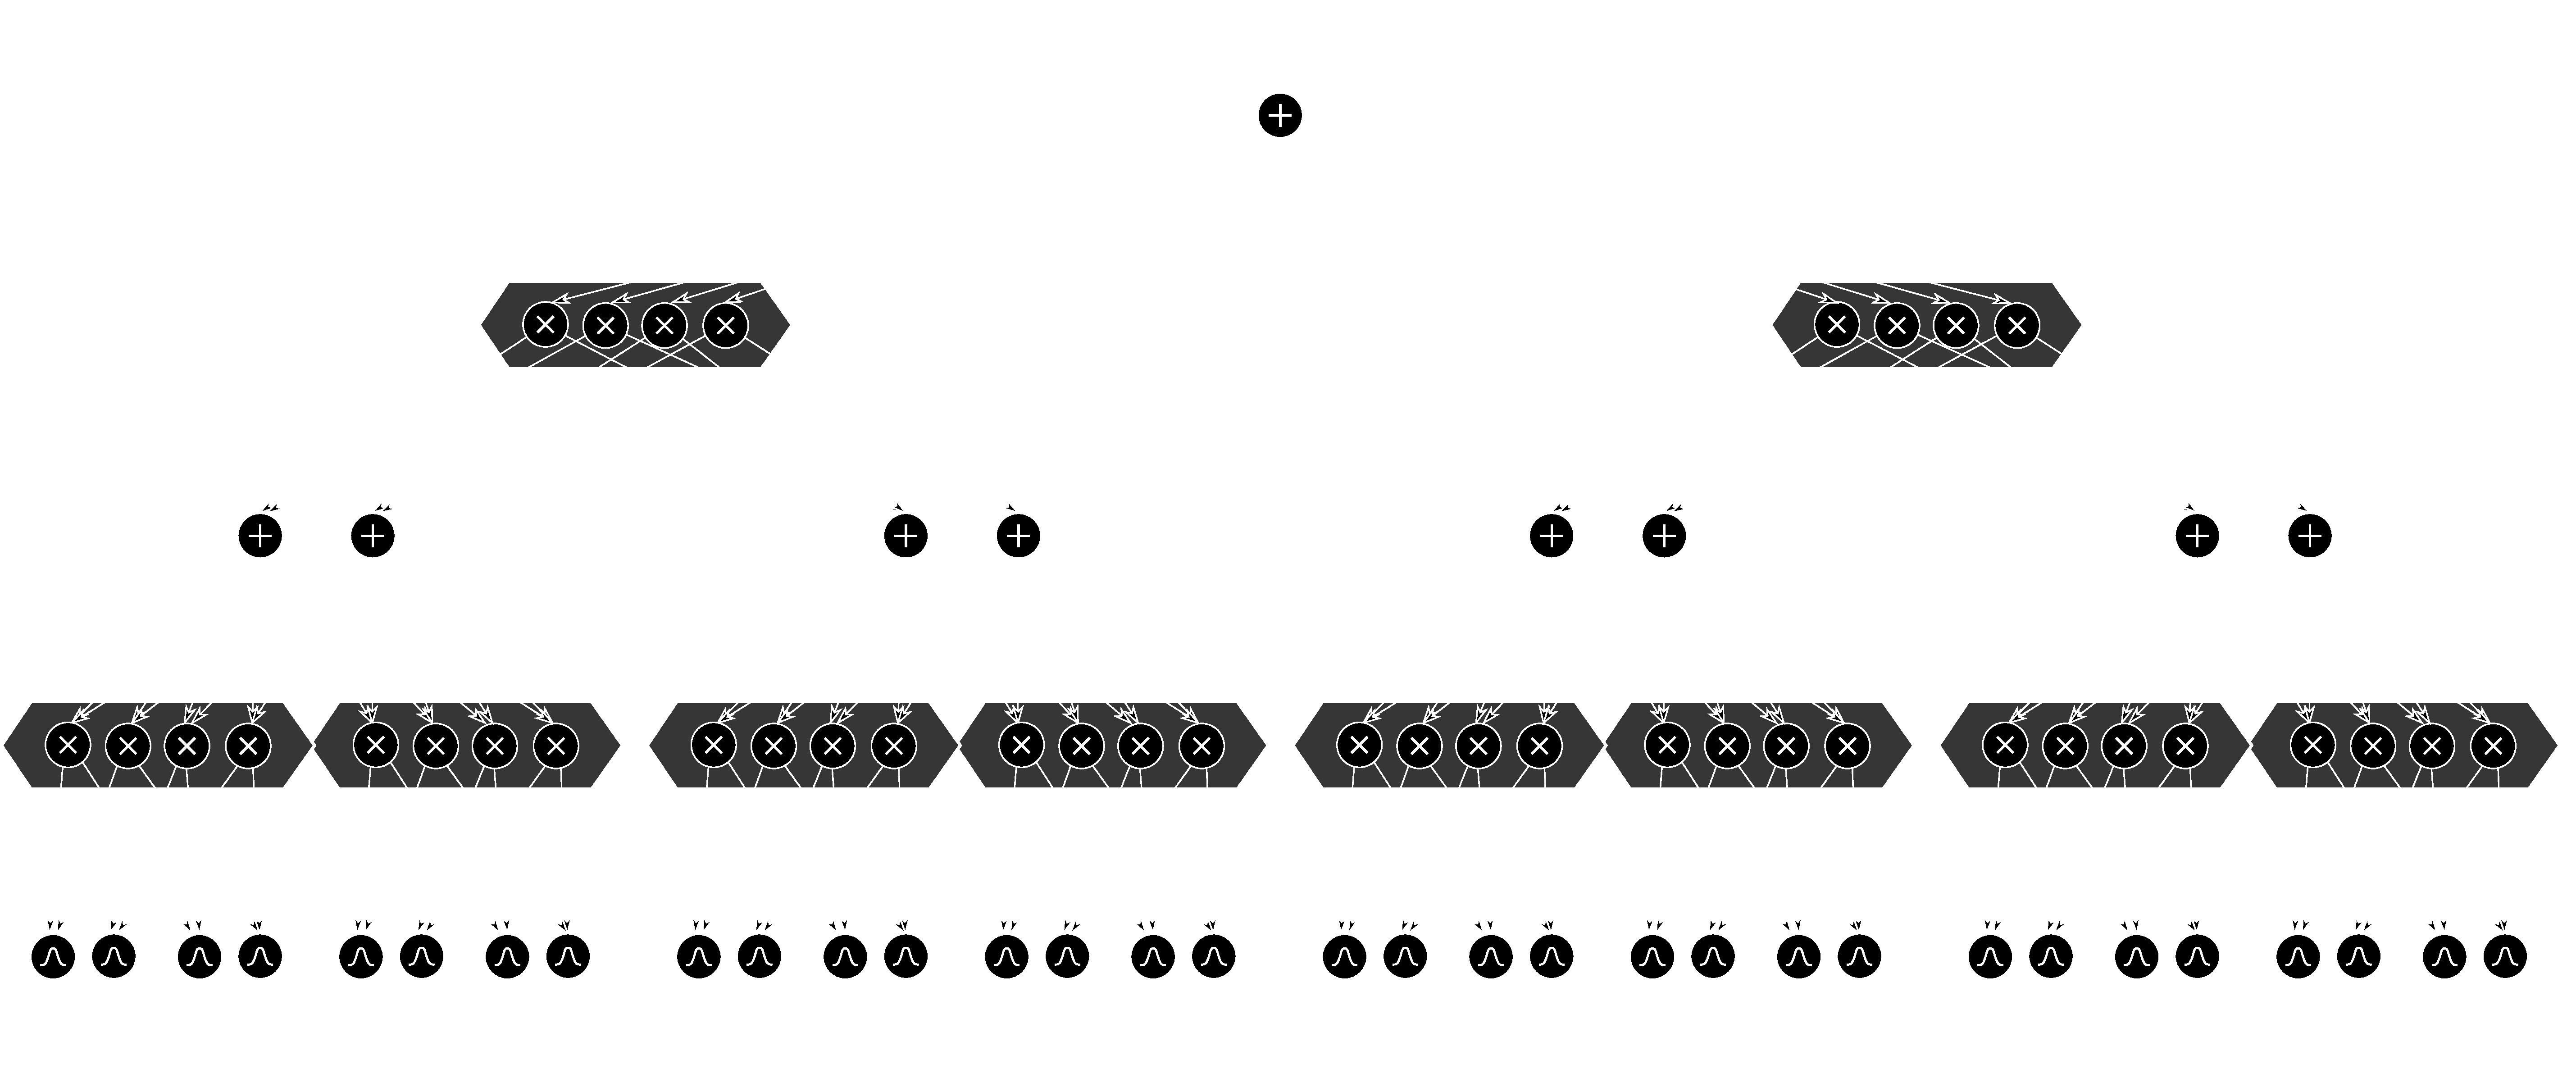
\includegraphics[width=0.9\linewidth]{region-graph}
%  \caption{Example region-graph. Based on the illustration by [Peharz2019].}
%\end{figure}
%
%\end{frame}

\begin{frame}{Bayesian Structure}
    \begin{block}{Why care about Bayesian structure learning?}

\begin{itemize}
        \item Competitive results.
        \item Occam's razor effect prevents overfitting.
        \item Works on heterogeneous data domains
        \item We can use nonparametric formulations, e.g.~infinite SPNs.
        \item Can be used in cases of missing values, by using exact marginalisation of missing values.
    \end{itemize}
\end{block}
\end{frame}

\begin{frame}{Bayesian Structure}
%\begin{itemize}
%    \item We assume $\graph$ is a tree-shaped region graph, i.e., the SPN is a \emph{not} a tree.
%    \item For each dimension $d$ we introduce a latent variable $Y_{\partition,d}$ at each partition node (bucket of product nodes).
%    \item The latent variables represent an assign of $d$ to a child, given a unique path leading to the node.
%\end{itemize}

\begin{figure}
    \centering
    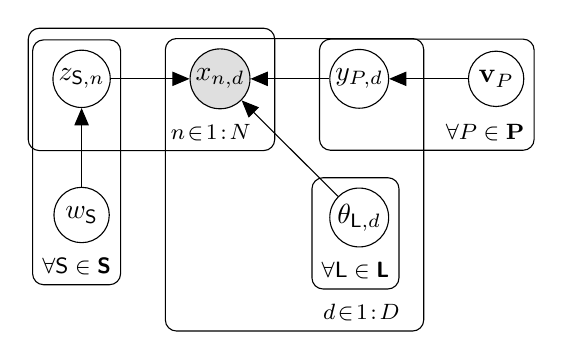
\begin{tikzpicture}
        \node[obs] (x) {$\xnd$};
        \node[latent, left=of x] (z) {$z_{\SumNode,n}$};
        \node[latent, right=of x] (y) {$y_{\partition,d}$};
        \node[latent, below=of y] (t) {$\theta_{\Leaf,d}$};
        \node[latent, below=of z] (w) {$w_{\SumNode}$};
        \node[latent, right=of y] (o) {$\vp_{\partition}$};

        \edge {z,t} {x} ; %
        \edge {y} {x} ; %
        \edge {w} {z} ; %
        \edge {o} {y} ; %

        \plate {zs} {(z)(w)} {$\forall \SumNode \in \SumNodes$} ;
        \plate {yo} {(y)(o)} {$\forall \partition \in \partitions$} ;
        \plate {t} {(t)} {$\forall \Leaf \in \Leaves$} ;
        \plate [inner xsep=0.3cm] {xyt} {(x)(y)(t)} {$d\!\in\!1\!:\!D$} ;
        \plate [inner xsep=0.3cm] {xz} {(x)(z)(xyt.north west)} {$n\!\in\!1\!:\!N$} ;
    \end{tikzpicture}
    \caption{Generative model for Bayesian structure learning.}\label{fig:BSPN}
\end{figure}
\end{frame}

\begin{frame}{Bayesian Structure}
Posterior inference can be performed using ancestral within Gibbs sampling.

\begin{figure}
    \centering
    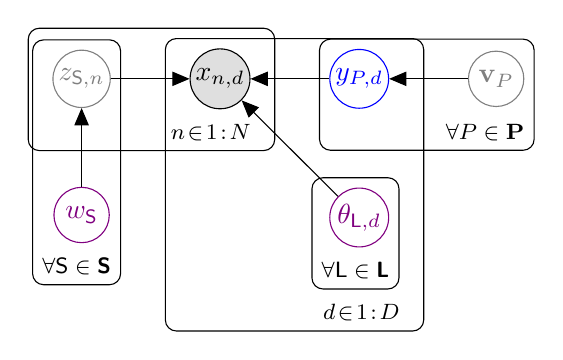
\begin{tikzpicture}
        \node[obs] (x) {$\xnd$};
        \node[gray, latent, draw=gray, left=of x] (z) {$z_{\SumNode,n}$};
        \node[blue, latent, draw=blue, right=of x] (y) {$y_{\partition,d}$};
        \node[violet, latent, draw=violet, below=of y] (t) {$\theta_{\Leaf,d}$};
        \node[violet, latent, draw=violet, below=of z] (w) {$w_{\SumNode}$};
        \node[gray, latent, draw=gray, right=of y] (o) {$\vp_{\partition}$};

        \edge {z,t} {x} ; %
        \edge {y} {x} ; %
        \edge {w} {z} ; %
        \edge {o} {y} ; %

        \plate {zs} {(z)(w)} {$\forall \SumNode \in \SumNodes$} ;
        \plate {yo} {(y)(o)} {$\forall \partition \in \partitions$} ;
        \plate {t} {(t)} {$\forall \Leaf \in \Leaves$} ;
        \plate [inner xsep=0.3cm] {xyt} {(x)(y)(t)} {$d\!\in\!1\!:\!D$} ;
        \plate [inner xsep=0.3cm] {xz} {(x)(z)(xyt.north west)} {$n\!\in\!1\!:\!N$} ;
    \end{tikzpicture}
    \caption{Generative model for Bayesian structure and learning.}\label{fig:BSPN}
\end{figure}
\end{frame}

\begin{frame}{Bayesian Structure - Missing Values Experiment}
Performance under increasing amount of missing values (missing completely at random).
\begin{center}
    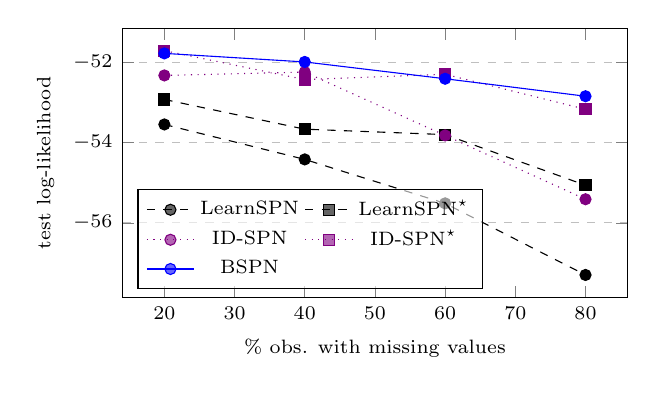
\begin{tikzpicture}
%
\begin{axis}[
%
    width=8cm,
%
    height=5cm,
%
    xlabel={\scriptsize{\% obs. with missing values}},
%
    ylabel={\scriptsize{test log-likelihood}},
%
    legend pos=south west,
    legend columns=2,
    legend style={font=\scriptsize},
    legend image post style={scale=1},
    legend style={fill opacity=0.6, draw opacity=1,text opacity=1},
    label style={font=\scriptsize},
    tick label style={font=\scriptsize},
%
    ymajorgrids=true,
%
    grid style=dashed
]

\addplot [color=black, dashed, mark=*, mark options={solid}] coordinates {
    (20, -53.551654150378006)
%
    (40, -54.421205612626615)
%
    (60, -55.51437111821264)
%
    (80, -57.29533673640321)
%
    };
%
\addlegendentry{LearnSPN}

%
\addplot [color=black, dashed, mark=square*, mark options={solid}] coordinates {
    (20, -52.9306308300396)
%
    (40, -53.669159658525054)
%
    (60, -53.804286870223166)
%
    (80, -55.06448194755978)
%
    };
%
\addlegendentry{LearnSPN$^\star$}
%

%
\addplot [color=violet, dotted, mark=*, mark options={solid}] coordinates {
    (20, -52.332443930626056)
%
    (40, -52.24919890693739)
%
    (60, -53.824333727580374)
%
    (80, -55.41192445685279)
%
    };
%
\addlegendentry{ID-SPN}

%
\addplot [color=violet, dotted, mark=square*, mark options={solid}] coordinates {
    (20, -51.71630289170897)
%
    (40, -52.4355408358714)
%
    (60, -52.30368237732657)
%
    (80, -53.173612370558374)
%
    };
%
\addlegendentry{ID-SPN$^\star$}

\addplot [color=blue, solid, mark=*, mark options={solid}] coordinates {
    (20, -51.784)
%
    (40, -51.997)
%
    (60, -52.415)
%
    (80, -52.85)
%
    };
%
\addlegendentry{BSPN}

%
\end{axis}
%
\end{tikzpicture}
\end{center}
\end{frame}


%
%\begin{frame}{Experiments (missing data)}
%\begin{figure}
%  \begin{minipage}{.48\textwidth}
%     \begin{tikzpicture}
%
%\begin{axis}[
%
%    width=5.5cm,
%
%    height=4cm,
%
%    xlabel={\scriptsize{\% obs. with missing values}},
%
%    ylabel={\scriptsize{test log-likelihood}},
%
%    legend pos=south west,
%    legend columns=2,
%    legend style={font=\tiny},
%    legend image post style={scale=0.5},
%    legend style={fill=background, draw=white, fill opacity=0.6, draw opacity=1,text opacity=1},
%    label style={font=\tiny},
%    tick label style={font=\tiny},
%
%    ymajorgrids=true,
%
%    grid style=dashed,
%
%    cycle list name=my black white
%
%]
%
%\addplot coordinates {
%
%    (20, -53.551654150378006)
%
%    (40, -54.421205612626615)
%
%    (60, -55.51437111821264)
%
%    (80, -57.29533673640321)
%
%    };
%
%\addlegendentry{LearnSPN}
%
%
%\addplot coordinates {
%
%    (20, -52.9306308300396)
%
%    (40, -53.669159658525054)
%
%    (60, -53.804286870223166)
%
%    (80, -55.06448194755978)
%
%    };
%
%\addlegendentry{LearnSPN$^\star$}
%
%
%
%\addplot coordinates {
%
%    (20, -52.332443930626056)
%
%    (40, -52.24919890693739)
%
%    (60, -53.824333727580374)
%
%    (80, -55.41192445685279)
%
%    };
%
%\addlegendentry{ID-SPN}
%
%
%\addplot coordinates {
%
%    (20, -51.71630289170897)
%
%    (40, -52.4355408358714)
%
%    (60, -52.30368237732657)
%
%    (80, -53.173612370558374)
%
%    };
%
%\addlegendentry{ID-SPN$^\star$}
%
%\addplot coordinates {
%
%    (20, -51.784)
%
%    (40, -51.997)
%
%    (60, -52.415)
%
%    (80, -52.85)
%
%    };
%
%\addlegendentry{BSPN}
%
%
%\end{axis}
%
%\end{tikzpicture}
%\caption{EachMovie (D: 500, N: 5526)}
%\end{minipage}
%\begin{minipage}{.48\textwidth}
%  \begin{tikzpicture}
%
%\begin{axis}[
%
%    width=5.5cm,
%
%    height=4cm,
%
%    xlabel={\scriptsize{\% obs. with missing values}},
%
%    legend pos=north east,
%
%    ymajorgrids=true,
%
%    grid style=dashed,
%    label style={font=\tiny},
%    tick label style={font=\tiny},
%
%    cycle list name=my black white,
%
%]
%
%\addplot coordinates {
%
%    (20, -161.41130223478262)
%
%    (40, -163.56351684466114)
%
%    (60, -162.96930286251663)
%
%    (80, -168.00941901059738)
%
%    };
%
%\addlegendentry{learnSPN}
%
%
%
%
%\addplot coordinates {
%
%    (20, -161.4285603783307)
%
%    (40, -165.36322925292424)
%
%    (60, -164.87160515320465)
%
%    (80, -164.53405856701238)
%
%    };
%
%\addlegendentry{learnSPN$^\star$}
%
%
%
%\addplot coordinates {
%
%    (20, -152.1845925143198)
%
%    (40, -154.95268171360382)
%
%    (60, -158.58576871121716)
%
%    (80, -165.45426630310263)
%
%    };
%
%\addlegendentry{ID-SPN}
%
%
%\addplot coordinates {
%
%    (20, -152.26143497732696)
%
%    (40, -153.5671636300716)
%
%    (60, -153.5671636300716)
%
%    (80, -157.2684578353222)
%
%    };
%
%\addlegendentry{ID-SPN$^\star$}
%
%\addplot coordinates {
%
%    (20, -157.078)
%
%    (40, -157.876)
%
%    (60, -158.625)
%
%    (80, -159.123)
%
%    };
%
%\addlegendentry{BSPN}
%  \legend{}; % empty the legend so as not to print it
%
%\end{axis}
%
%\end{tikzpicture}
%\caption{WebKB (D: 839, N: 3361)}
%\end{minipage}
%\begin{minipage}{.5\textwidth}
%  \begin{tikzpicture}
%
%\begin{axis}[
%
%    width=5.5cm,
%
%    height=4cm,
%
%    xlabel={\scriptsize{\% obs. with missing values}},
%
%    legend pos=north east,
%
%    ymajorgrids=true,
%
%    grid style=dashed,
%    label style={font=\tiny},
%    tick label style={font=\tiny},
%
%    cycle list name=my black white
%
%]
% 
%
%\addplot coordinates {
%
%    (20, -250.83622675798426)
%
%    (40, -261.1124401206212)
%
%    (60, -266.0005946312015)
%
%    (80, -273.39617177834293)
%
%    };
%
%\addlegendentry{learnSPN}
%
%
%
%\addplot coordinates {
%
%    (20, -284.24099564475125)
%
%    (40, -261.6701870807035)
%
%    (60, -265.4755544697035)
%
%    (80, -297.06332858812755)
%
%    };
%
%\addlegendentry{learnSPN$^\star$}
%
%
%
%\addplot coordinates {
%
%    (20, -250.68554855757577)
%
%    (40, -253.81061585454546)
%
%    (60, -261.81913693030305)
%
%    (80, -272.27580261212125)
%
%    };
%
%\addlegendentry{ID-SPN}
%
%
%
%\addplot coordinates {
%
%    (20, -249.82204944242426)
%
%    (40, -252.33469486666664)
%
%    (60, -254.56216942424243)
%
%    (80, -256.8125317606061)
%
%    };
%
%\addlegendentry{ID-SPN$^\star$}
%
%\addplot coordinates {
%
%    (20, -251.551)
%
%    (40, -254.101)
%
%    (60, -255.551)
%
%    (80, -256.144)
%
%    };
%
%\addlegendentry{BSPN}
%  \legend{}; % empty the legend so as not to print it
%
%\end{axis}
%
%\end{tikzpicture}
%\caption{BBC (D: 1058, N: 1895)}
%\end{minipage}
%\end{figure}
%
%\end{frame}


% --
% Applications
% --
\section{Applications}

\begin{frame}{Existing Applications}
There exist several applications of SPNs in various fields:
\begin{itemize}
    \item Computer vision, e.g.~image classification, medical image processing, attend-infer-repeat.
    \item Language processing, e.g.~language modelling, bandwidth extension.
    \item Robotics, e.g.~semantic mapping.
    \item Nonlinear regression, and many more\footnote{\scriptsize https://github.com/arranger1044/awesome-spn\#applications}
\end{itemize}
\end{frame}

\begin{frame}{SPNs for Regression}
We have recently\footnote{\scriptsize M. Trapp et al.: Deep structured mixtures of Gaussian processes. To appear at AISTATS, 2020.} introduced a combination of SPNs with Gaussian processes, which yields an interesting nonparametric regression model that allows exact and efficient posterior inference.

Our model can be understood as an exponentially large mixture over naive-local-experts of Gaussian processes.
\end{frame}

\begin{frame}{Deep Structured Mixtures of GPs}
    A Gaussian Process (GP) is a collection of random variables $F$ indexed by an arbitrary
    covariate space $X$, where any finite subset of $F$ is Gaussian distributed.

    A GP can be understood as a prior over functions.

    \begin{figure}
        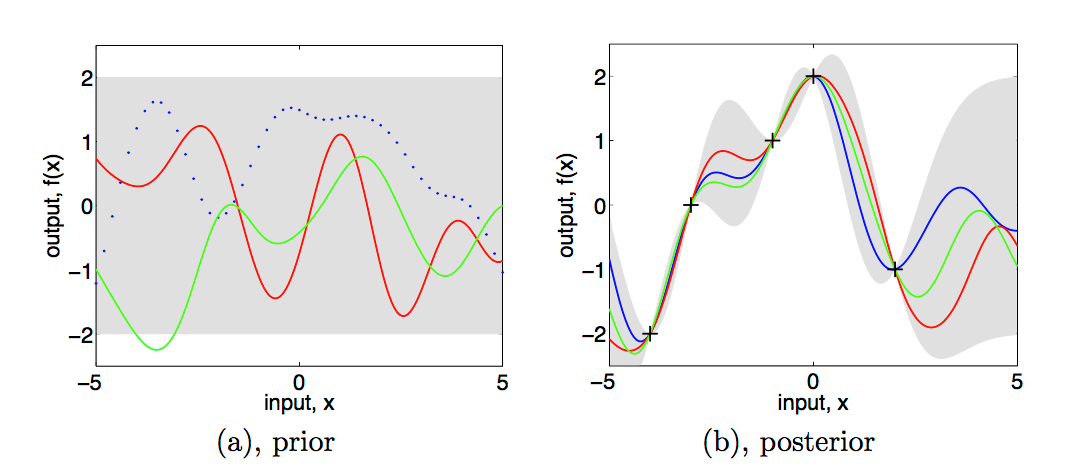
\includegraphics[width=0.9\textwidth]{GP_Rasmussen}
        \caption{\scriptsize C. E. Rasmussen \& C. K. I. Williams, Gaussian Processes for Machine Learning, 2006.}
    \end{figure}
\end{frame}


\begin{frame}{}

\centering
Thank you for your attention!

\end{frame}

\end{document}
